\section{Aleatoric uncertainty}

The first uncertainty type analyzed is the aleatoric. As said before, this uncertainty refers to the stochasticity in process modeled by the BNN. Therefore, it is a good candidate as quantity to use to determine if the network is sure or not about a prediction since it depends from the input data. The aleatoric uncertainty is computed as:
\[
	aleatoric = diag\{\frac{1}{T} \sum_{t=1}^{T} [diag(\hat{p}_t) - \hat{p}_t^{\otimes 2}]\}
\]

where $T$ is the number of predictions made for the same input, and $p_t$ is the $t^{th}$ prediction.

A key point is the determination of the threshold value. In order to do this, the upper and lower values of this uncertainty  were determined:

\begin{itemize}
	\item Case minimum uncertainty: This happens when $\hat{p}$ has all terms equal to 0 except one which is 1, and its position identifies the predicted class. Applying the formula, it results in $aleatoric = 0$, that aligns the hypothesis made. 
	\item Case maximum uncertainty: The prediction is uncertain at the maximum level when $\hat{p}$ has only equal values. In particular the value is $\frac{1}{m}$, where m is the number of classes to predict. In this case the uncertainty is $aleatoric = \frac{m-1}{m^2}$, for this specific case study $m = 10$, therefore $aleatoric = 0.09$.
\end{itemize}

Given the upper and lower bounds, a linear interpolation is employed to calculate the threshold value based on the desired confidence level. This method allows for the estimation of an appropriate threshold that aligns with the desired confidence level. 

\[
	threshold = 0.09 * (1 - conf \_ level), \ with \ con \_ level \in [0,1]
\]


To evaluate this approach, a series of experimental simulations were conducted to examine the changes in accuracy and the number of unknown values obtained. The results are shown in \Fig~\ref{fig:aleatoric_class}.

\Fig~\ref{fig:aleatoric_acc} illustrates the variation in accuracy as the confidence level increases. It is evident that the accuracy improves as the confidence level rises, primarily because the network provides predictions with higher certainty.

\Fig~\ref{fig:aleatoric_unk} shows the trend of the unknown ratio, which increases as well. This is due to the fact that the network outputs more unknown values as the confidence level increases. At a confidence level of 1, all samples are discarded, since the aleatoric uncertainty could have very small but non-zero values.

\begin{figure}[h]
	\centering
	\begin{subfigure}{.5\textwidth}
		\centering
		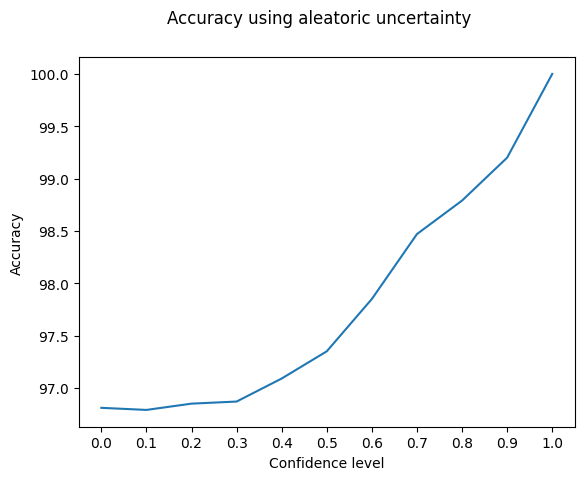
\includegraphics[width=0.8\linewidth]{ImageFiles/ClassifUncer/aleatoric_acc}
		\caption{Accuracy trend when the confidence level is increased}
		\label{fig:aleatoric_acc}
	\end{subfigure}%
	\begin{subfigure}{.5\textwidth}
		\centering
		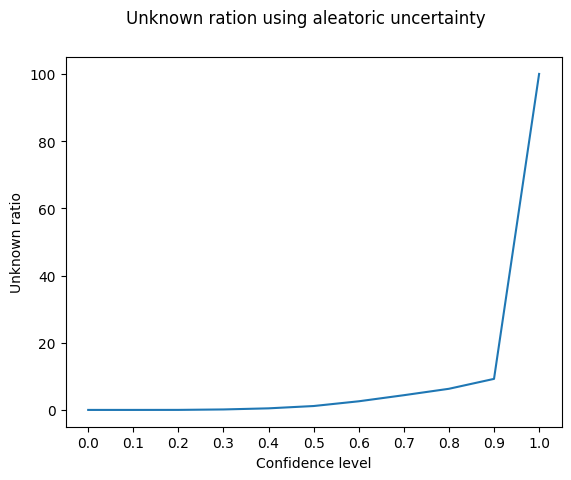
\includegraphics[width=0.8\linewidth]{ImageFiles/ClassifUncer/aleatoric_unk}
		\caption{Unknown ratio trend when the confidence level is increased}
		\label{fig:aleatoric_unk}
	\end{subfigure}
	\caption{Performances of the BNN using the aleatoric uncertainty during classification}
	\label{fig:aleatoric_class}
\end{figure}

Setting $conf \_ level = 1$ renders the approach ineffective as the network will only produce unknown values, rendering the predictions useless. This arises the need to find a balance between the confidence level and the number of unknowns, which is a consideration for the specific task. In non-critical applications, opting for a low confidence level might be preferable. In such cases, obtaining a prediction, even if it turns out to be incorrect, is prioritized due to the potential high economic consequences associated with halting the system. On the other hand, in critical applications, like the medical field, ensuring certainty in decisions becomes paramount. If the network lacks confidence in its predictions, it is essential to pause the decision-making process and request the intervention of a qualified expert, such as a doctor, to ensure accuracy and mitigate potential risks.